\title{Kalibrierung des 3D Scanners}

\documentclass[a4letter,10pt]{scrartcl}
\usepackage{a4wide}

% deutsche Silbentrennung
\usepackage[ngerman]{babel}

\usepackage{amssymb}

% wegen deutschen Umlauten
\usepackage[applemac]{inputenc}

% Kein Einr�cken zu Beginn eines Absatzes
\setlength\parindent{0pt}

%% Special tabular version
\usepackage{tabularx}

\usepackage{graphicx}
\usepackage{subfigure}


\begin{document}

\author{Prof. Dr. Philipp Jenke, Joschka Schulz} 
\title{Kalibrierung des 3D Scanners} 
\date{} 
\maketitle

In diesem Dokument wird der Ansatz zur Kalibrierung des 3D Scanners beschrieben. Der Aufbau des Scanners ist in Abbildung \ref{fig:setup} dargestellt. Ziel der Kalibrierung ist es, Informationen aus verschiedenen Koordinatensystemen in ein einheitliches Koordinatensystem (Weltkoordinatensystem) zu bringen. Unter Koordinatensystem wird hier ein Tupel bestehend aus einer Rotationmatrix $R \in \mathbb{R}^{3x3}$ und einem Translationsvektor $\mathbf{t} \in \mathbb{R}^3$ verstanden. Die Spalten der Rotationsmatrix sind gleichzeitig die Basisvektoren (Koordinatenachsen) des Koordinatensystems. Es handelt sich jeweils um orthonormale Systeme, d.h. die Basisvektoren haben die L�nge $1$ und stehen jeweils paarweise senkrecht aufeinander.

\begin{figure}[ht]
\centering
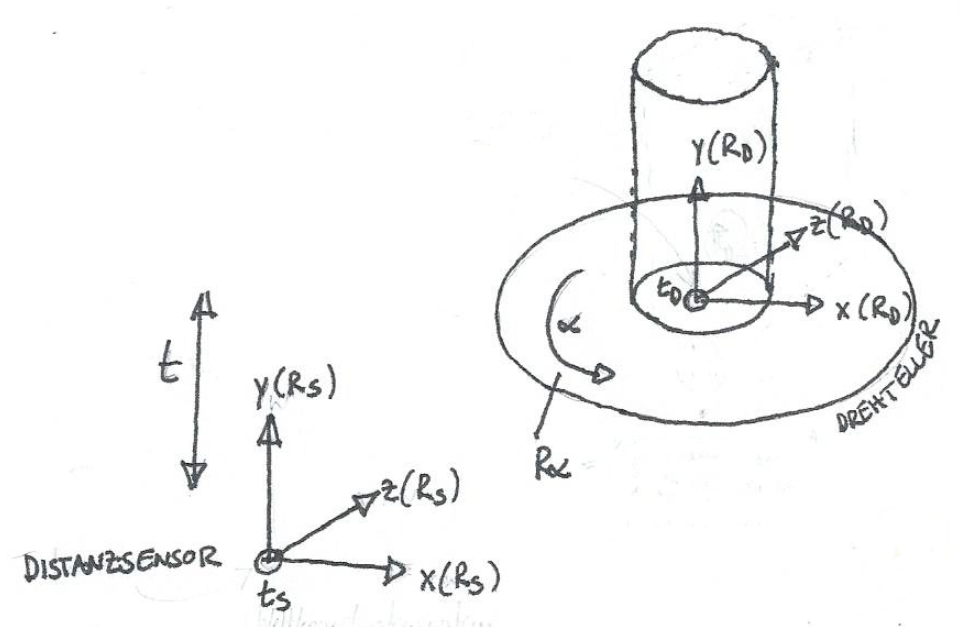
\includegraphics[height=8cm]{setup.png}
\caption{Setup des 3D Scanners bestehend aus je einem Koordinatensystem f�r den Sensor ($S$) und f�r den Drehteller ($D$).}
\label{fig:setup}
\end{figure}

\section{Koordinatensysteme}

Der Distanzsensor ist auf einer vertikal verschiebbaren Plattform angebracht. F�r das Koordinatensystem des Sensors verwenden wir den Bezeichner $S$ (f�r Sensor). Das Koordinatensystem besteht also aus der Rotationsmatrix $R_S$ und dem Translationsvektor $\mathbf{t_S}$. Wir definieren, dass der Sensor in Richtung der $\mathbf{z}$-Achse ausgerichtet ist, die Translationsplattform bewegt sich entlang der $\mathbf{y}$-Achse. Ein Messpunkt $\mathbf{p_M}$ ergibt sich aus der gemessenen Entfernung $z_0$ und dem aktuellen Translationswert $t_0$:
$$\mathbf{p_M} = \left(\begin{array}{c}0 \\ t_0 \\ z_0 \\ \end{array} \right).$$
Ein Messpunkt wird folgenderma�en in das Euklidische Koordinatensystem transformiert:
$$\mathbf{p_E} = R_S \cdot p_M + \mathbf{t_S}$$

Der rotierende Drehteller befindet sich im Koordinatensystem $D$, bestehend aus der Rotationsmatrix $R_D$ und dem Translationsanteil $\mathbf{t_D}$. Au�erdem dreht sich der Drehteller. Bei jeder Messung hat er eine Position $\alpha$ eingenommen. Die Rotation um den Winkel $\alpha$ wird durch die Rotationsmatrix $R_{\alpha}$ beschrieben. Wir nehmen hier an, dass sich der Drehteller im Ursprung des Weltkoordinatensystems befindet, daher ist $\mathbf{t_D}$ der Nullvektor:
$$\mathbf{t_D} = \mathbf{0} =  \left(\begin{array}{c}0 \\ 0 \\0 \\ \end{array} \right).$$
Ein Punkt $\mathbf{p_E}$ aus dem Euklidischen Koordinatensystem wird also in Drehtellerkoordinaten (und damit Weltkoordinaten) folgenderma�en umgerechnet:
$$\mathbf{p_D} = R_{\alpha} \cdot R^{-1}_D \cdot (\mathbf{p_E} - \mathbf{t_D}).$$

Daraus ergibt sich folgende Vorschrift f�r die Umrechnung eines Me�punktes $\mathbf{p_M}$ in Drehttellerkoordinaten: 
$$\mathbf{p_D} = R_{\alpha} \cdot R^{-1}_D \cdot (R_S \cdot \mathbf{p_M} + \mathbf{t_S} -\mathbf{t_D}).$$

\section{Kalibrierung}

Bei der Kalibrierung m�ssen die Unbekannten der beiden Koordinatensysteme bestimmt werden. Wir nehmen hier vereinfachend an, dass die $\mathbf{x}$-, $\mathbf{y}$- und $\mathbf{z}$-Achsen der beiden Koordinatensysteme identisch sind\footnote{{\bf Anmerkung:} f�r $\mathbf{x}$ und $\mathbf{z}$ ist das zun�chst keine Einschr�nkung. Es k�nnte aber sein, dass die beiden $\mathbf{y}$-Achsen nicht in die exakt gleiche Richtung zeigen. Hier ist langfristig eine Erweiterung der Kalibrierung notwenig. Dann m�ssen auch die $\mathbf{x}$- und die $\mathbf{z}$-Achse angepasst werden.}.

Daher muss zun�chst nur der Translationsanteil $\mathbf{t_S}$ des Sensorkoordinatensystems bestimmt werden. Die Verschiebung entlang der $\mathbf{y}$-Achse ist irrelevant, daher sind nur ${t_S}_{|x}$ und ${t_S}_{|Z}$ zu bestimmen. Die Kalibrierung erfolgt �ber die Aufnahme eines bekannten Objektes, in diesem Fall eines Zylinders. Ein Zylinder l�sst sich beschreiben durch
\begin{itemize}
\item Richtungsvektor $\mathbf{d_Z} \in \mathbb{R}^3$
\item beliebiger Punkt auf der Achse $\mathbf{p_Z} \in \mathbb{R}^3$
\item Radius $r_Z \in \mathbf{R}$
\end{itemize}
Die Hauptachse des Zylinders zeigt hier in die $\mathbf{y}$-Richtung (siehe Abbildung \ref{fig:setup}), daher:
$$\mathbf{d_Z} = \left(\begin{array}{c}0 \\ 1 \\0 \\ \end{array} \right).$$

Die $y$-Koordinate des Zylinderpunktes ist wieder irrelevant, ${p_Z}_{|x}$ und ${p_Z}_{|z}$ sind aber vorher nicht bekannt und m�ssen daher im Rahmen der Kalibrierung bestimmt werden. 

Die grundlegende Idee der Kalibrierung ist es, Belegungen f�r die Unbekannten zu finden, sodass alle gescannten Messungen auf der Oberfl�che des Zylinders liegen. Dazu ben�tigt man eine Anstandsfunktion $dist_Z(\mathbf{p})$ von der Oberfl�che des Zylinders:
$$ dist_Z(\mathbf{p}) = || ( \mathbf{p_z} + ((\mathbf{p} - \mathbf{p_Z}) \cdot \mathbf{d_Z} ) \cdot \mathbf{d_Z} ) - \mathbf{p} ||.$$

Mit Hilfe der Distanzfunktion l�sst sich eine Fehlerfunktion $E$ bestimmen ("Wie weit sind die Messpunkte im Schnitt von der Oberfl�che entfernt?"):
$$E(\mathbf{x}) = \frac{1}{n} \sum_{i \in n} dist_Z(\mathbf{{p_i}_D})^2,$$
f�r einen Scan mit $n$ Messpunkten $\mathbf{{p_i}_D}$, die jeweils ins Drehtellerkoordinatensystem umgerechnet wurden.

Ziel ist es, das Minimum dieser Fehlerfunktion zu finden, also Werte f�r die Unbekannten $\mathbf{x} = ({t_S}_{|x}, {t_S}_{|x}, {p_Z}_{|x}, {p_Z}_{|z})$, sodass $$E(\mathbf{x}) \rightarrow \min.$$

Wir verwenden hier ein naives Gradientenabstiegsverfahren. Wir bilden also den Gradienten der Fehlerfunktion $E(\mathbf{x})$:
$$\mathbf{\nabla E} = \left(\begin{array}{c} \frac{\partial{E}}{\partial{{t_S}_{|x}}} \\ \frac{\partial{E}}{\partial{{t_S}_{|z}}} \\ \frac{\partial{E}}{\partial{{p_Z}_{|x}}} \\ \frac{\partial{E}}{\partial{{p_Z}_{|Z}}} \\ \end{array} \right)$$

Iterativ finden wir dann eine bessere L�sung f�r den Parametervektor $\mathbf{x}$ durch die Vorschrift
$$\mathbf{x_{i+1}} = \mathbf{x_i} - \mathbf{\nabla E} \cdot h$$
f�r eine geeignet kleine Schrittweite $h$. Als Abbruchbedingung f�r die Iteration sind verschiedene Verfahren denkbar (manuelle Steuerung, �berwachung des Fehlers, �berwachung der Ver�nderung zwischen zwei Schritten, ...)

Die partiellen Ableitungen f�r die Berechnung des Gradienten werden �ber finite Differenzen approximiert.

\end{document}